\section{Pré-étude} \label{sec:Pre-Etude}

\subsection{Fonctionnement du système} \label{ssec:Fonctionnement}

\subsubsection{Schéma bloc} \label{sssec:Schema-bloc}
\begin{figure}[h]
	\centering
	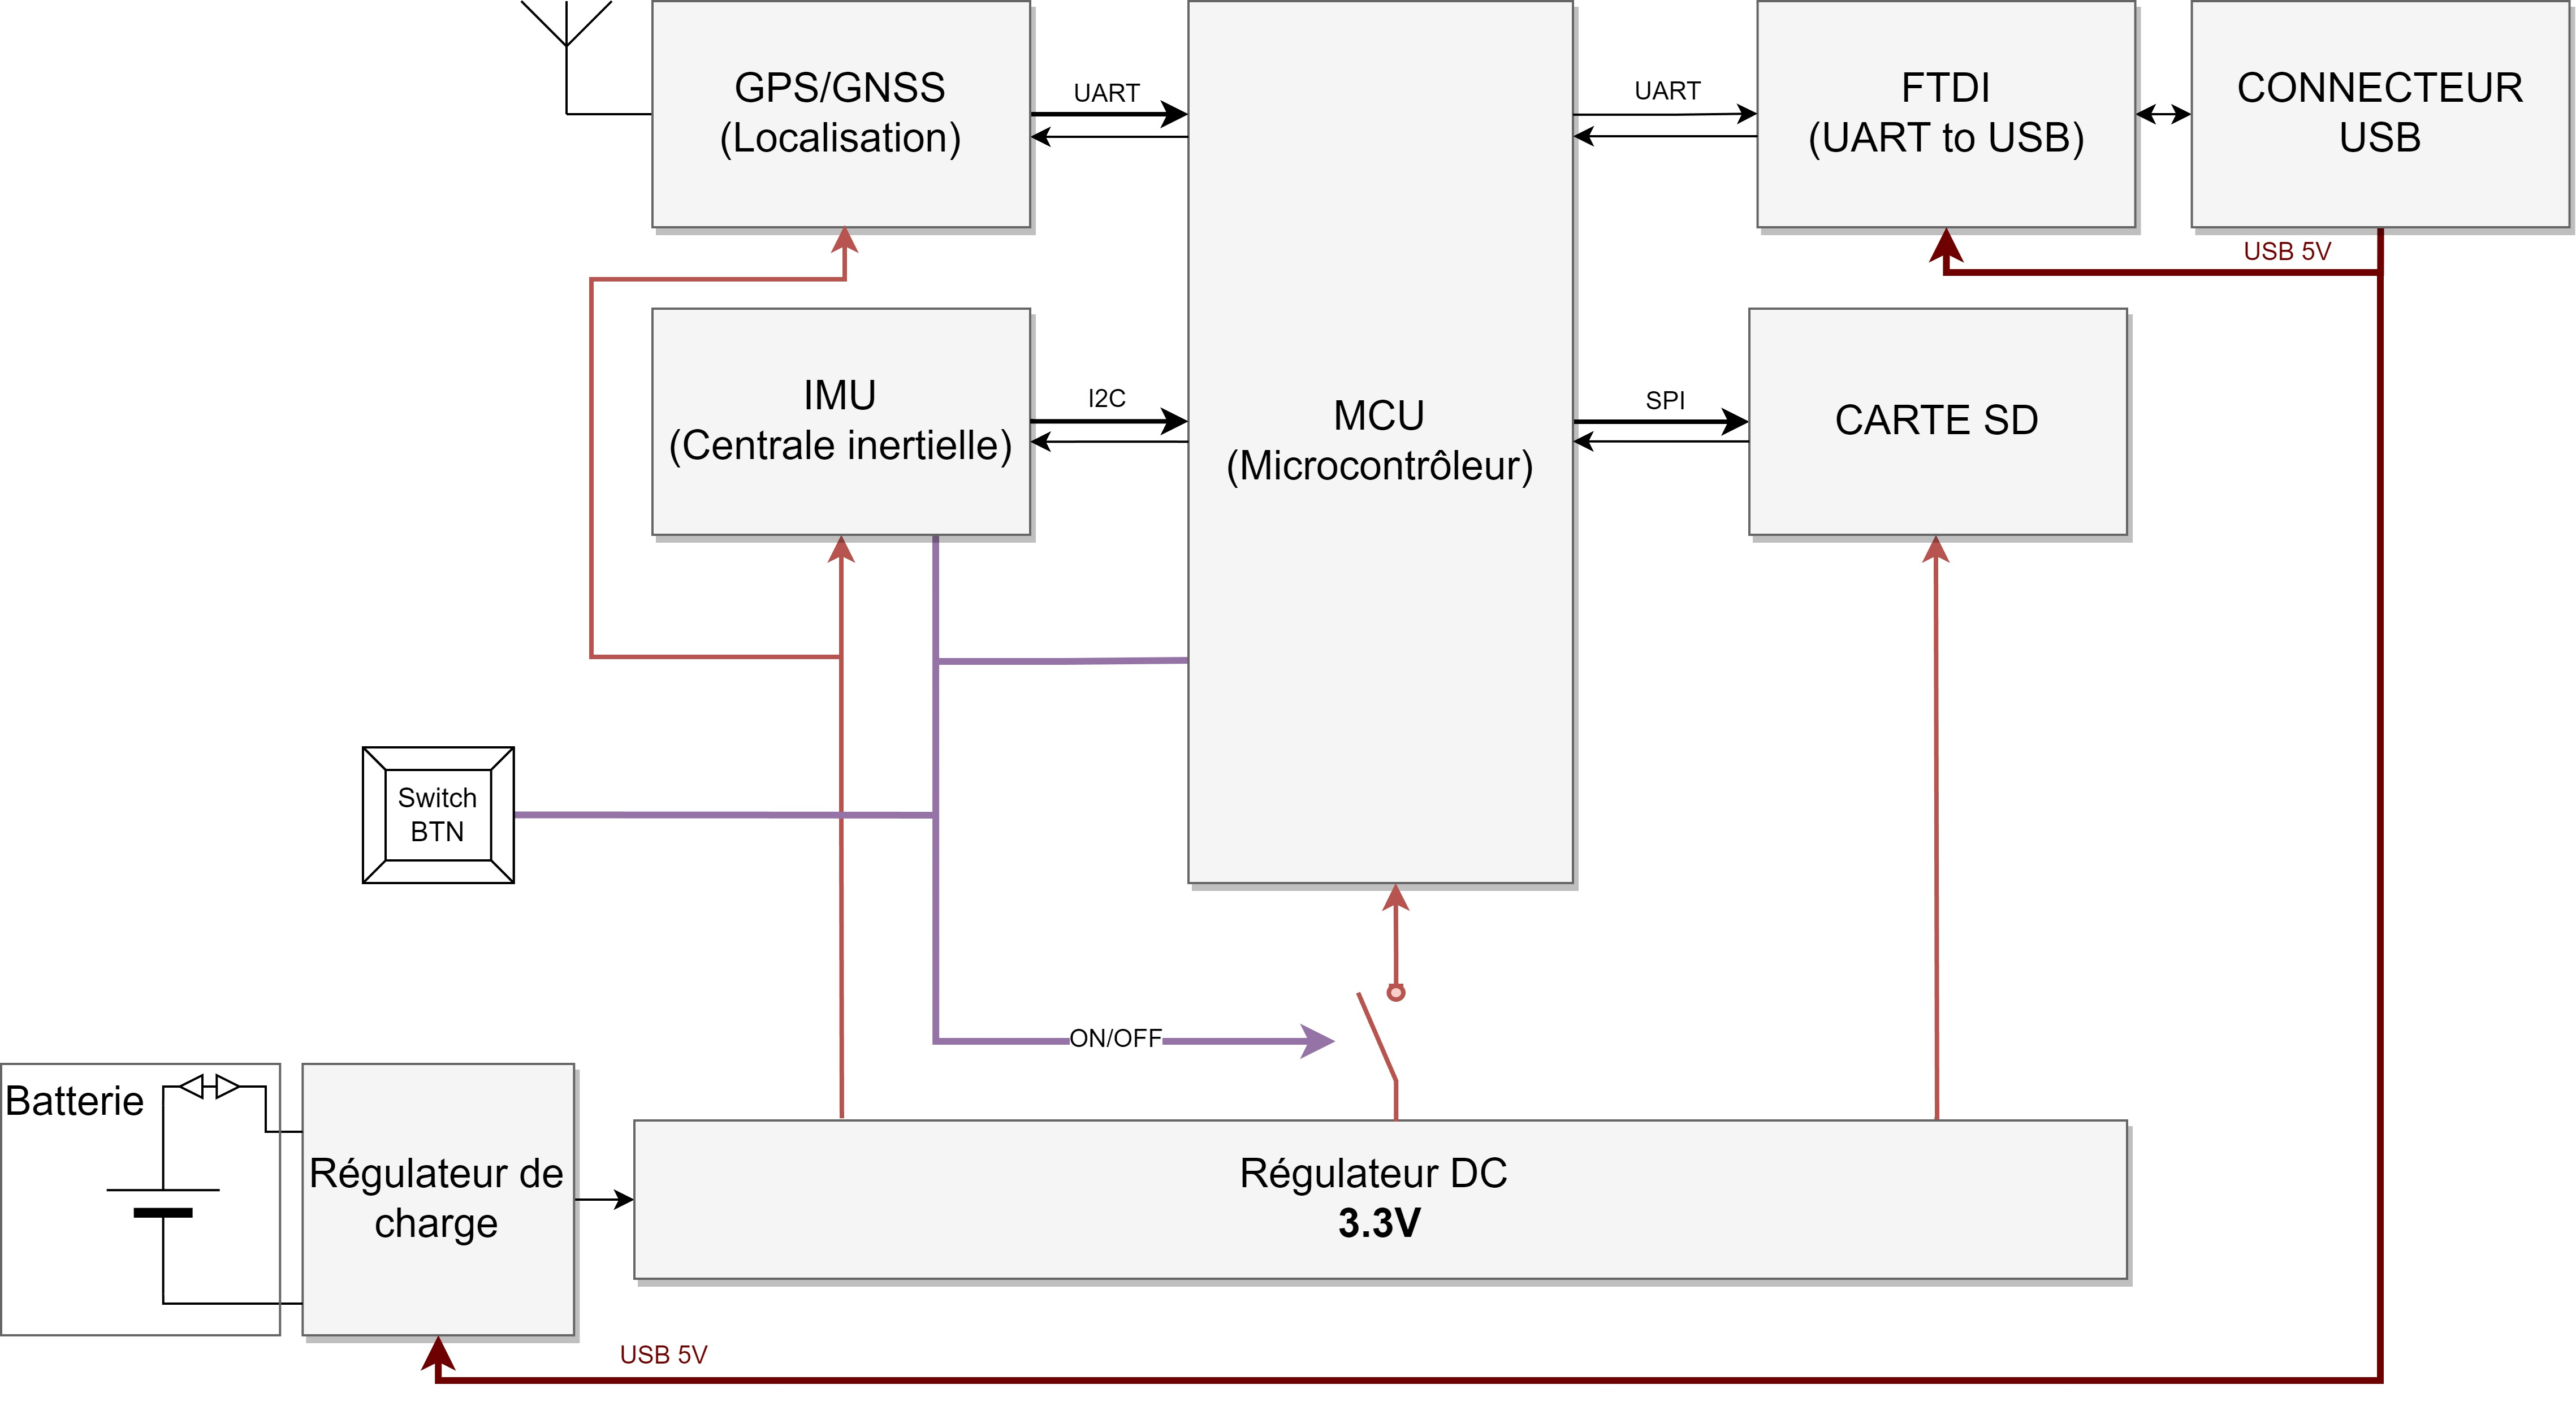
\includegraphics[width=1\textwidth]{../figures/cdc/blocs_grossiers_no_antenna.jpg}
	\caption{Schéma de principe}
	\label{fig:blocsgrossiers}
	\source{Auteur}
\end{figure}
% ---- Description des blocs ----
\subsection{Description des blocs}

\begin{table}[h]
	\resizebox{\columnwidth}{!}{%
		\begin{tabular}{|l|l|}
			\hline
			Bloc         & Description                                                                         \\ \hline
			\Gls{gnss}.  & Récepteur \Gls{rf} avec antenne interne/externe et communication UART.              \\ \hline
			\Gls{mcu}.   & Microcontrôleur PIC32, intelligence du système, basse consommation.                 \\ \hline
			\Gls{imu}.   & Centrale inertielle, accélération, gyroscope...                                     \\ \hline
			Carte SD     & Stockage des données de vol.                                                        \\ \hline
			\Gls{FTDI}.  & Convertis la communication USB en série.                                            \\ \hline
			Régulateurs. & Le régulateur de charge gère la charge de l'accu. et un régulateur 3.3V le suit.    \\ \hline
			Batterie.    & La batterie est un accu que l'on peut charger par USB et permet une bonne autonomie. \\ \hline
		\end{tabular}%
	}
\end{table}

\subsection{Choix des composants} \label{ssec:Choix-composant}

\subsubsection{Microcontrôleur} \label{sssec:Choix-MCU}

\subsubsection{Centrale inertielle} \label{sssec:Choix-Centrale-inertielle}

\subsubsection{GPS / GNSS} \label{sssec:Choix-GPS}

\subsubsection{Transmetteur radio-fréquence} \label{sssec:Choix-Rft}
NEC IR transmission protocol

\subsubsection{Batterie, charge et régulation} \label{sssec:Choix-Batterie-charge}

\subsection{Estimation des coûts} \label{sssec:Estimation-Couts}
